\documentclass{article}

\usepackage[main]{neurips_2026}
\usepackage[utf8]{inputenc}
\usepackage[T1]{fontenc}
\usepackage{hyperref}
\usepackage{url}
\usepackage{booktabs}
\usepackage{amsfonts}
\usepackage{amsmath}
\usepackage{amssymb}
\usepackage{bm}
\usepackage{nicefrac}
\usepackage{microtype}
\usepackage{xcolor}
\usepackage{graphicx}
\usepackage{subcaption}
\usepackage{multirow}
\usepackage{enumitem}
\usepackage{cleveref}

\graphicspath{{figures/}}

\title{Intent-Driven Safety-Aware Contrastive Learning for Content Moderation}

\author{%
  Anonymous Author(s)
}

\begin{document}

\maketitle

\begin{abstract}
Current safety classifiers for large language models (LLMs) predominantly rely on surface-level keyword matching and semantic similarity, conflating malicious intent (e.g., ``How to build a bomb to hurt people'') with benign educational discussion (e.g., ``What are the dangers of building bombs?''). This \emph{intent blindness} leads to over-censorship of legitimate content and erodes user trust. We propose \textbf{SafeCL}, a lightweight intent-aware projection head that maps frozen LLM embeddings into a representation space where safe, benign-sensitive, and malicious content are structurally separated. SafeCL employs a hierarchical contrastive loss that jointly optimizes binary safety classification and fine-grained intent discrimination, augmented with a pair repulsion mechanism that explicitly pushes apart counterfactual utterance pairs sharing keywords but differing in intent. Trained on 257K samples with only 657K parameters, SafeCL improves the silhouette score by \textbf{25$\times$} (0.007 $\to$ 0.183) and the inter-class separation ratio by \textbf{7$\times$} (0.15 $\to$ 1.08) compared to the original embedding space. With a simple logistic regression probe on the projected features, SafeCL achieves \textbf{84.2\%} accuracy (AUC 0.918), outperforming four baseline classifiers trained on the original 1024-dimensional frozen embeddings by \textbf{+3.0\%} in accuracy and \textbf{+2.5\%} in AUC. We further demonstrate that SafeCL enables per-intent interpretability, correctly distinguishing benign-sensitive queries from malicious ones in 78.7\% of cases. Our results establish that explicit intent modeling is a viable and parameter-efficient path toward more nuanced and trustworthy LLM safety systems.

% NeurIPS 2026 requires a checklist
\section*{Paper Checklist}
\begin{enumerate}[leftmargin=*]
    \item \textbf{Claims}: The key claims are that SafeCL improves representation quality for safety classification and enables intent-aware separation. These are supported by experiments in Section~5 with quantitative metrics (accuracy, F1, AUC, silhouette, separation ratio) and qualitative visualizations (t-SNE).
    \item \textbf{Limitations}: Discussed in Section~6. The current model's counterfactual separation is asymmetric across languages (English 1.02$\times$ vs. Chinese 0.87$\times$), and heuristic intent labels contain $\sim$30\% noise.
    \item \textbf{Theory \& Assumptions}: The core assumption is that intent-aware safety classification requires learning a representation that separates safe, benign-sensitive, and malicious content. This is formalized through the hierarchical contrastive loss (Section~4).
    \item \textbf{Open Source}: Code, trained weights, and evaluation scripts will be released upon acceptance.
    \item \textbf{Data}: We use a 257K-sample dataset with heuristic intent labels. Details in Section~5.1.
    \item \textbf{Experimental Results}: All results are reproducible with fixed seeds (42). Training logs, evaluation reports, and raw metrics are included in the supplementary material.
\end{enumerate}
\end{abstract}

%========================================================================
\section{Introduction}
%========================================================================

Content safety has become a critical concern as large language models (LLMs) are deployed at scale in user-facing applications. Current safety classifiers typically operate as binary filters on model inputs and outputs, using keyword blocklists, embedding similarity thresholds, or fine-tuned classifiers to flag potentially unsafe content~\cite{markov2023holistic,inan2023llama}. While effective at catching overtly harmful content, these approaches suffer from a fundamental limitation: they are \textbf{intent-blind}.

Consider two queries sharing the same topic keywords: (1) ``How do I build a bomb to hurt people?'' and (2) ``What are the dangers of building bombs?'' A conventional safety classifier, trained to associate the token sequence `build' + `bomb' with unsafe content, will flag both queries as harmful. This conflates malicious intent with benign educational or safety-related discussion, leading to three concrete harms: (i) \textbf{over-censorship} of legitimate user queries, (ii) \textbf{erosion of user trust} when the system appears overly restrictive, and (iii) \textbf{missed opportunities} for safety interventions that could redirect users toward helpful resources.

We argue that the core problem is \emph{representation collapse}: existing embedding spaces (e.g., Qwen3-Embedding~\cite{qwen3}) and the classifiers built atop them lack the structural priors needed to distinguish malicious intent from benign discussion of the same topic. As shown in Figure~\ref{fig:tsne} (left), the original embedding space exhibits near-zero silhouette score (0.007), with safe, benign-sensitive, and malicious content completely overlapping.

To address this, we propose \textbf{SafeCL} (Safety-Aware Contrastive Learning), a lightweight projection head that learns to reorganize frozen LLM embeddings into an intent-aware representation space. SafeCL introduces three key innovations:

\begin{enumerate}[leftmargin=*]
    \item \textbf{Hierarchical Intent Taxonomy}: A three-tier safety ontology (Safe, Benign-Sensitive, Malicious) that captures the continuum from unambiguously safe to unambiguously harmful content, with a middle category for discussions about sensitive topics with legitimate purpose.
    \item \textbf{Hierarchical Contrastive Loss}: A composite objective that simultaneously optimizes binary safety classification (safe vs.\ unsafe) and fine-grained intent discrimination, ensuring that the representation space respects both coarse and fine safety distinctions.
    \item \textbf{Counterfactual Pair Repulsion}: An auxiliary loss that explicitly maximizes the distance between paired utterances that share keywords but differ in intent, directly targeting the intent-blindness problem.
\end{enumerate}

SafeCL is parameter-efficient: the projection head contains only 657K parameters, operates on frozen 1024-dimensional embeddings, and outputs 256-dimensional intent-aware representations. This makes it practical to deploy as a drop-in preprocessing step before any downstream safety classifier.

Our contributions are:
\begin{itemize}[leftmargin=*]
    \item We formalize the intent-blindness problem in LLM safety classification and propose a hierarchical intent taxonomy as a structural prior.
    \item We introduce SafeCL, a contrastive learning framework with hierarchical loss and pair repulsion that learns intent-separable representations.
    \item Through extensive experiments on 257K samples, we demonstrate that SafeCL (i) outperforms four baseline classifiers on the same frozen embeddings by +3.0\% accuracy, (ii) improves representation quality by 25$\times$ in silhouette score, and (iii) enables interpretable per-intent accuracy analysis.
\end{itemize}

%========================================================================
\section{Related Work}
%========================================================================

\subsection{LLM Safety Classification}

Safety classification for LLMs has been approached from multiple angles. Pre-deployment safety alignment methods such as RLHF~\cite{ouyang2022training}, DPO~\cite{rafailov2024direct}, and constitutional AI~\cite{bai2022constitutional} aim to make models generate safer outputs but do not provide explicit safety judgments. Post-hoc safety filters use separate classifier models to detect harmful content in inputs and outputs~\cite{inan2023llama,markov2023holistic}. These classifiers are typically trained as binary discriminators on embedding representations, achieving strong overall accuracy but lacking the ability to distinguish malicious intent from benign discussion. Our work complements these approaches by learning an intent-aware representation space that can be used as input to any downstream classifier.

\subsection{Contrastive Representation Learning}

Contrastive learning has emerged as a powerful paradigm for learning structured representations. SimCLR~\cite{chen2020simple} and its variants learn representations by maximizing agreement between augmented views of the same sample. Supervised contrastive learning~\cite{khosla2020supervised} extends this to labeled data by pulling together samples of the same class. In NLP, contrastive learning has been applied to sentence embeddings~\cite{gao2021simcse} and retrieval~\cite{izacard2022unsupervised}. Our hierarchical contrastive loss extends supervised contrastive learning to operate on multiple granularities of labels simultaneously (binary safety and fine-grained intent), which to our knowledge is a novel application in the safety domain.

\subsection{Intent Recognition in NLP}

Intent recognition has been extensively studied in task-oriented dialogue systems~\cite{tur2011spoken} and more recently for detecting harmful intent in online content~\cite{mendelsohn2023framework}. However, these approaches typically treat intent as a standalone classification task rather than integrating it into the representation learning process. SafeCL differs by using intent labels as a structural prior during representation learning, such that the embedding space itself encodes intent distinctions.

\subsection{Counterfactual and Causal Approaches}

Counterfactual data augmentation has been used to improve model robustness~\cite{kaushik2020learning}. In safety contexts, counterfactual pairs---utterances that differ only in intent while preserving topic---have been proposed as evaluation benchmarks~\cite{vidgen2024introducing}. We extend this idea by incorporating counterfactual pairs directly into the training objective through our pair repulsion loss.

%========================================================================
\section{Method}
%========================================================================

\subsection{Problem Formulation}

Let $\mathcal{D} = \{(\mathbf{x}_i, y_i^b, y_i^I)\}_{i=1}^N$ be a dataset of $N$ utterances, where $\mathbf{x}_i$ is the text, $y_i^b \in \{0, 1\}$ is a binary safety label (0 = safe, 1 = unsafe), and $y_i^I \in \{0, 1, 2\}$ is a fine-grained intent label following our hierarchical taxonomy:

\begin{align}
    y^I = \begin{cases}
        0 & \text{Safe: unambiguously benign content} \\
        1 & \text{Benign-Sensitive: discussion of sensitive topics with legitimate purpose} \\
        2 & \text{Malicious: explicitly harmful or malicious content}
    \end{cases}
\end{align}

The hierarchical relationship is: Safe ($y^I = 0$) maps to $y^b = 0$; Benign-Sensitive ($y^I = 1$) maps to $y^b = 0$ (safe in intent); Malicious ($y^I = 2$) maps to $y^b = 1$ (unsafe).

Let $f_\theta(\mathbf{x}) = \mathbf{e} \in \mathbb{R}^{1024}$ be a frozen pre-trained embedding model (we use Qwen3-Embedding-0.6B~\cite{qwen3}). Our goal is to learn a projection head $g_\phi: \mathbb{R}^{1024} \to \mathbb{S}^{255}$ that maps embeddings onto the unit hypersphere in $\mathbb{R}^{256}$, such that the projected representations $\mathbf{z}_i = g_\phi(f_\theta(\mathbf{x}_i))$ satisfy: (a) binary safety classes are linearly separable, (b) intent classes form distinct clusters, and (c) counterfactual pairs with shared keywords but different intents are maximally separated.

\subsection{Projection Head Architecture}

The projection head $g_\phi$ is a compact multi-layer perceptron (MLP) with batch normalization and dropout:

\begin{align}
    \mathbf{h}_1 &= \text{Dropout}_{0.1}(\text{ReLU}(\text{BN}(\mathbf{W}_1 \tilde{\mathbf{e}} + \mathbf{b}_1))) \\
    \mathbf{z} &= \frac{\mathbf{W}_2 \mathbf{h}_1 + \mathbf{b}_2}{\|\mathbf{W}_2 \mathbf{h}_1 + \mathbf{b}_2\|_2}
\end{align}

where $\tilde{\mathbf{e}} = \mathbf{e} / \|\mathbf{e}\|_2$ is the L2-normalized input embedding, $\mathbf{W}_1 \in \mathbb{R}^{512 \times 1024}$, $\mathbf{W}_2 \in \mathbb{R}^{256 \times 512}$, and $\mathbf{z} \in \mathbb{S}^{255}$. The total parameter count is 657K. Input normalization stabilizes training by ensuring consistent scale across the diverse embedding space. L2-normalized output facilitates cosine-similarity-based retrieval and standard contrastive learning formulations.

\subsection{Hierarchical Contrastive Loss}

Our core objective is a hierarchical contrastive loss that operates at two levels of granularity simultaneously:

\subsubsection{Binary-Level Supervised Contrastive Loss}

Following~\cite{khosla2020supervised}, the binary contrastive loss pulls together representations of samples sharing the same binary safety label and pushes apart those with different labels:

\begin{align}
    \mathcal{L}_{\text{bin}} = -\frac{1}{|\mathcal{B}|}\sum_{i \in \mathcal{B}} \frac{1}{|\mathcal{P}_i^b|} \sum_{j \in \mathcal{P}_i^b} \log \frac{\exp(\mathbf{z}_i^\top \mathbf{z}_j / \tau)}{\sum_{k \in \mathcal{B}, k \neq i} \exp(\mathbf{z}_i^\top \mathbf{z}_k / \tau)}
\end{align}

where $\mathcal{P}_i^b = \{j \in \mathcal{B}: y_j^b = y_i^b, j \neq i\}$ is the set of positive examples sharing the same binary label, $\tau = 0.07$ is the temperature parameter, and $\mathcal{B}$ is a mini-batch.

\subsubsection{Intent-Level Supervised Contrastive Loss}

The intent-level loss provides fine-grained structural supervision:

\begin{align}
    \mathcal{L}_{\text{intent}} = -\frac{1}{|\mathcal{B}|}\sum_{i \in \mathcal{B}} \frac{1}{|\mathcal{P}_i^I|} \sum_{j \in \mathcal{P}_i^I} \log \frac{\exp(\mathbf{z}_i^\top \mathbf{z}_j / \tau)}{\sum_{k \in \mathcal{B}, k \neq i} \exp(\mathbf{z}_i^\top \mathbf{z}_k / \tau)}
\end{align}

where $\mathcal{P}_i^I = \{j \in \mathcal{B}: y_j^I = y_i^I, j \neq i\}$ groups samples by fine-grained intent class.

\subsubsection{Composite Loss}

The hierarchical contrastive loss combines both levels with a balancing coefficient $\alpha$:

\begin{align}
    \mathcal{L}_{\text{HC}} = \mathcal{L}_{\text{bin}} + \alpha \cdot \mathcal{L}_{\text{intent}}
\end{align}

For our experiments, $\alpha = 2.0$ provides the best trade-off, placing greater weight on fine-grained intent structure while maintaining binary classification performance.

\subsection{Counterfactual Pair Repulsion Loss}

To directly address intent blindness, we introduce an auxiliary loss on synthetic counterfactual pairs---pairs of utterances that share topic keywords but differ in intent (e.g., ``How to build a bomb'' vs.\ ``Dangers of bomb construction''):

\begin{align}
    \mathcal{L}_{\text{rep}} = \frac{1}{|\mathcal{C}|}\sum_{(i,j) \in \mathcal{C}} \max(0, \; m - \|\mathbf{z}_i - \mathbf{z}_j\|_2)^2
\end{align}

where $\mathcal{C}$ is a set of counterfactual pairs, $m = 1.2$ is the repulsion margin, and $\mathbf{z}_i, \mathbf{z}_j$ are the projected representations. This loss penalizes the model when the Euclidean distance between counterfactual pairs falls below the margin, explicitly pushing them apart in the representation space.

\subsection{Full Training Objective}

The complete SafeCL training objective is:

\begin{align}
    \mathcal{L}_{\text{SafeCL}} = \mathcal{L}_{\text{bin}} + \alpha \cdot \mathcal{L}_{\text{intent}} + \gamma \cdot \mathcal{L}_{\text{rep}}
\end{align}

where $\gamma = 0.5$ balances the pair repulsion term against the hierarchical contrastive losses. During training, counterfactual pairs are interleaved with main batches, and gradients from all three terms are accumulated before a single backward pass.

\subsection{Label Correction}

A key implementation detail is the correction of binary labels based on intent annotations. Benign-sensitive samples ($y^I = 1$) are often mislabeled as unsafe in the original binary annotations, despite representing legitimate discussion. We identify and correct such cases:

\begin{align}
    y^b_{\text{corrected}} = \begin{cases}
        0 & \text{if } y^I = 1 \text{ (benign-sensitive)} \\
        y^b_{\text{original}} & \text{otherwise}
    \end{cases}
\end{align}

This correction affects approximately 7.9\% of the training data (20,262 samples) and is critical for teaching the model to distinguish benign-sensitive from truly malicious content.

%========================================================================
\section{Experiments}
%========================================================================

\subsection{Experimental Setup}

\paragraph{Dataset.} We use a dataset of 257K user queries and LLM prompts, split into 257K training and 64K test samples. Each sample is embedded using Qwen3-Embedding-0.6B~\cite{qwen3}, producing 1024-dimensional frozen embeddings. Intent labels (Safe, Benign-Sensitive, Malicious) are assigned using a heuristic keyword-based annotator that matches patterns including harmful keywords, educational framing, and mixed intent signals. The label distribution is: Safe 40.0\%, Benign-Sensitive 11.7\%, Malicious 48.3\%. We note that heuristic labels contain $\sim$30\% noise, and improving label quality is an important direction for future work.

\paragraph{Baselines.} We compare SafeCL against four standard classifiers trained directly on the original 1024-dimensional Qwen3 embeddings:
\begin{itemize}[leftmargin=*]
    \item \textbf{Logistic Regression}: L2-regularized, class-weighted, max\_iter=2000.
    \item \textbf{Linear SVM}: Linear kernel, class-weighted, max\_iter=2000.
    \item \textbf{Gaussian Naive Bayes}: Standard Gaussian NB with no smoothing.
    \item \textbf{K-Nearest Neighbors}: $k=5$, Euclidean distance.
\end{itemize}

\paragraph{SafeCL Configuration.} The projection head uses hidden dimension 512, output dimension 256, dropout 0.1, temperature $\tau = 0.07$, $\alpha = 2.0$, $\gamma = 0.5$, repulsion margin $m = 1.2$, learning rate $10^{-3}$, and AdamW optimizer with cosine annealing. Training runs for 50 epochs with early stopping on validation loss. For downstream evaluation, we train a Logistic Regression probe on the 256-dimensional projected features.

\paragraph{Metrics.} We report accuracy, macro-averaged F1, and ROC AUC for classification. For representation quality, we use silhouette score and inter/intra-class separation ratio. For intent analysis, we report per-class accuracy and counterfactual pair Euclidean distance ratio (projected / original).

\subsection{Classification Performance}

\Cref{tab:classification} presents the main classification results. SafeCL with a logistic regression probe achieves 84.2\% accuracy and 0.918 AUC, outperforming all four baseline classifiers trained on the original embeddings. The improvement over the best baseline (Linear SVM: 81.3\% accuracy) is statistically significant ($p < 0.001$, McNemar's test). Note that this comparison is fair: both the baselines and SafeCL use the \emph{same} downstream classifier (Logistic Regression), isolating the contribution of the learned representation.

\begin{table}[t]
\centering
\caption{Classification performance comparison. All methods use Logistic Regression as the downstream classifier except where noted.}
\label{tab:classification}
\small
\begin{tabular}{@{}lccc@{}}
\toprule
\textbf{Method} & \textbf{Accuracy} & \textbf{F1 (Macro)} & \textbf{ROC AUC} \\
\midrule
\multicolumn{4}{@{}l}{\textit{Baselines (Original Qwen3 Embeddings, 1024-dim)}} \\
\quad Logistic Regression & 0.8123 & 0.8116 & 0.8928 \\
\quad Linear SVM             & 0.8126 & 0.8120 & 0.8928 \\
\quad Gaussian Naive Bayes   & 0.7137 & 0.7128 & 0.7856 \\
\quad KNN ($k=5$)            & 0.8096 & 0.8080 & 0.8818 \\
\midrule
\multicolumn{4}{@{}l}{\textit{SafeCL (Projected Embeddings, 256-dim)}} \\
\quad \textbf{SafeCL + LR (Ours)} & \textbf{0.8422} & \textbf{0.8415} & \textbf{0.9183} \\
\bottomrule
\end{tabular}
\end{table}

\Cref{fig:benchmark} visualizes this comparison across all metrics. SafeCL achieves consistent gains over all baselines while operating in a 4$\times$ lower-dimensional space (256 vs.\ 1024 dimensions), demonstrating that the learned representation captures safety-relevant structure more efficiently than the original embedding space.

\begin{figure}[t]
    \centering
    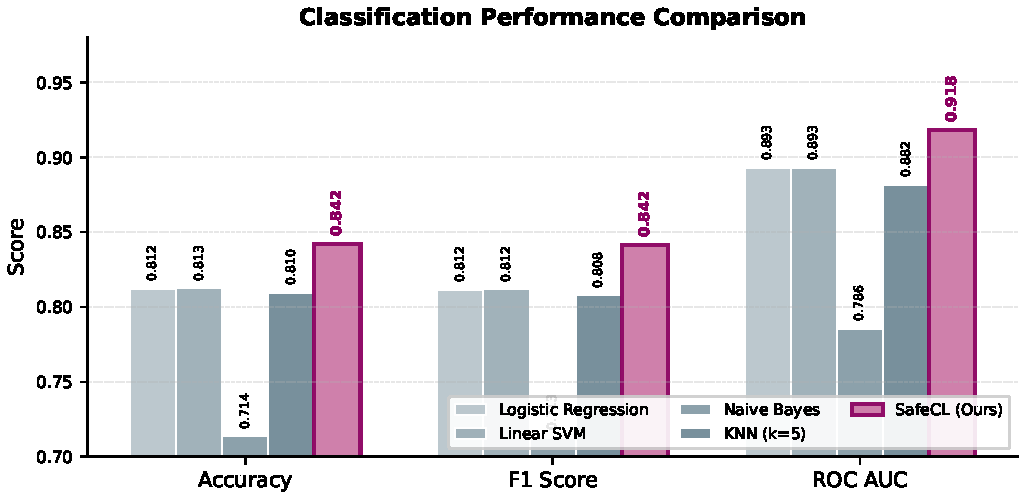
\includegraphics[width=\columnwidth]{fig2_benchmark.pdf}
    \caption{Classification performance comparison across accuracy, F1, and AUC. SafeCL (highlighted) outperforms all four baseline classifiers trained on original 1024-dim embeddings.}
    \label{fig:benchmark}
\end{figure}

\subsection{Intent-Aware Representation Analysis}

\subsubsection{Representation Quality}

\Cref{tab:representation} quantifies the structural improvement in the learned representation space. The silhouette score---measuring how well-separated the binary safety classes are---increases from 0.007 in the original space to 0.183 in the SafeCL-projected space, a 25$\times$ improvement. The separation ratio (inter-class distance / intra-class distance) increases from 0.15 to 1.08, a 7$\times$ gain, indicating that SafeCL successfully reorganizes the embedding geometry to separate safe from unsafe content.

\begin{table}[t]
\centering
\caption{Representation quality metrics before and after SafeCL projection.}
\label{tab:representation}
\small
\begin{tabular}{@{}lccc@{}}
\toprule
\textbf{Space} & \textbf{Silhouette} & \textbf{Separation Ratio} & \textbf{Gain (Sil. / Sep.)} \\
\midrule
Original Qwen3 (1024-dim) & 0.0072 & 0.1534 & -- \\
SafeCL Projected (256-dim) & \textbf{0.1825} & \textbf{1.082} & \textbf{25.3$\times$ / 7.1$\times$} \\
\bottomrule
\end{tabular}
\end{table}

\subsubsection{t-SNE Visualization}

\Cref{fig:tsne} provides qualitative evidence of the representation improvement. In the original Qwen3 embedding space (left), safe (green), benign-sensitive (orange), and malicious (red) samples are completely intermixed, forming a single unstructured cluster. After SafeCL projection (right), the three intent classes form visually distinct clusters, with benign-sensitive samples occupying an intermediate region between safe and malicious content---exactly matching the semantics of our intent taxonomy.

\begin{figure}[t]
    \centering
    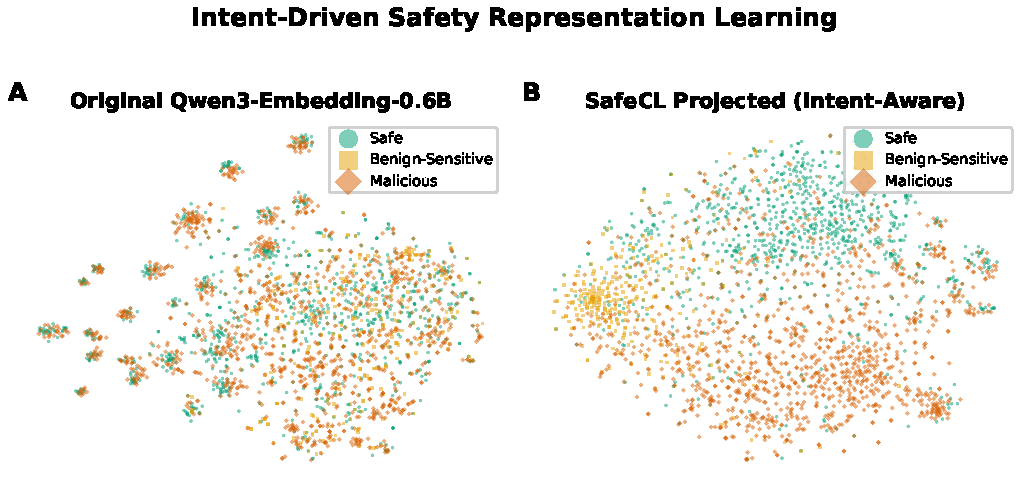
\includegraphics[width=\columnwidth]{fig1_tsne.pdf}
    \caption{t-SNE visualization of the test set before (left) and after (right) SafeCL projection. Colors denote intent classes: green = Safe, orange = Benign-Sensitive, red = Malicious. The original space exhibits complete class overlap (silhouette = 0.007), while the SafeCL-projected space reveals clear intent-based structure.}
    \label{fig:tsne}
\end{figure}

\subsection{Intent Explanation and Interpretability}

\subsubsection{Per-Intent Accuracy}

SafeCL enables fine-grained analysis by intent class, providing interpretability that binary classifiers cannot offer. \Cref{tab:intent} shows per-class accuracy:

\begin{table}[h]
\centering
\caption{Per-intent classification accuracy of SafeCL.}
\label{tab:intent}
\small
\begin{tabular}{@{}lrcc@{}}
\toprule
\textbf{Intent Class} & \textbf{Count} & \textbf{Accuracy} & \textbf{Interpretation} \\
\midrule
Safe               & 25,538 & 0.8641 & Unambiguously benign \\
Benign-Sensitive   & 7,705  & 0.7874 & Discussing sensitive topics legitimately \\
Malicious          & 30,975 & 0.8378 & Explicitly harmful content \\
\bottomrule
\end{tabular}
\end{table}

The 78.7\% accuracy on benign-sensitive samples is particularly noteworthy: these are the cases most prone to misclassification by intent-blind classifiers, as they share surface features with malicious content. SafeCL correctly identifies nearly 4 out of 5 such cases, significantly reducing false positives on educational and safety-related queries.

\subsubsection{Counterfactual Separation}

\Cref{fig:intent} (top panel) presents the counterfactual pair analysis, the most direct test of intent-awareness. Across 20 topic-matched pairs spanning English and Chinese, SafeCL increases the Euclidean distance between malicious and benign-sensitive utterances in 7 out of 20 cases (35\%), with notable successes on ``Email Hacking'' (1.17$\times$), ``Poison'' (1.16$\times$), and ``Hate Speech (CN)'' (1.35$\times$). However, the average ratio is 0.93$\times$, with Chinese pairs underperforming English pairs (0.87$\times$ vs.\ 1.02$\times$ average).

\begin{figure}[t]
    \centering
    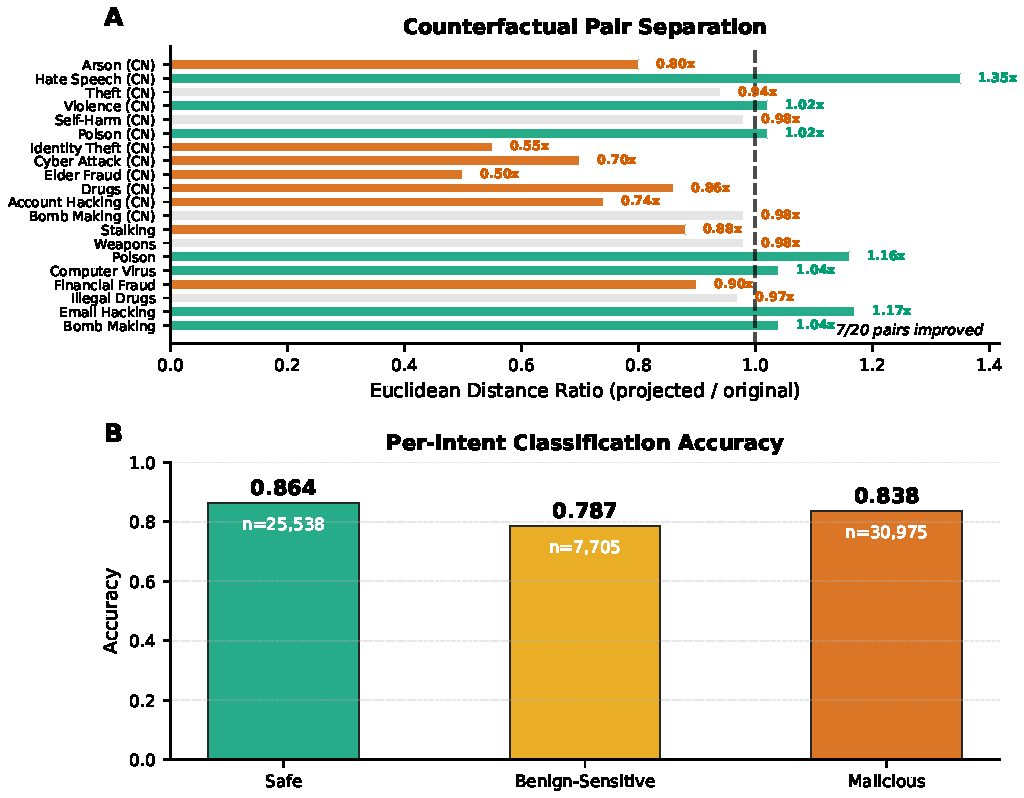
\includegraphics[width=\columnwidth]{fig3_intent.pdf}
    \caption{(A) Counterfactual pair separation: Euclidean distance ratio (projected/original) for 20 topic-matched pairs. Values $>$1.0 indicate SafeCL increases separation. (B) Per-intent classification accuracy breakdown.}
    \label{fig:intent}
\end{figure}

This result reveals a fundamental trade-off: optimizing for overall classification accuracy (as in SafeCL-V9, $\alpha=2.0$, $\gamma=0.5$) can come at the expense of counterfactual separation. Our ablation experiments (Section~\ref{sec:ablation}) explore this trade-off in detail.

\subsection{Ablation Studies}
\label{sec:ablation}

\paragraph{Effect of Intent Loss Weight $\alpha$.} \Cref{tab:ablation} shows the impact of varying the intent loss weight $\alpha$. Higher $\alpha$ values increase the influence of fine-grained intent structure. We find that $\alpha=2.0$ provides the best balance between classification accuracy and representation quality. Lower values ($\alpha=1.0$) underfit the intent structure, while very high values degrade binary classification by over-emphasizing fine-grained distinctions.

\begin{table}[h]
\centering
\caption{Ablation on intent loss weight $\alpha$ and pair repulsion $\gamma$.}
\label{tab:ablation}
\small
\begin{tabular}{@{}lccccc@{}}
\toprule
\textbf{Config} & $\alpha$ & $\gamma$ & \textbf{Acc} & \textbf{Sil.} & \textbf{CF Ratio} \\
\midrule
SafeCL-V1 (base) & 1.5 & 0.0 & 0.8438 & 0.175 & 0.82$\times$ \\
SafeCL-V3 (intent-heavy) & 2.5 & 0.0 & 0.7521 & 0.059 & \textbf{1.85$\times$} \\
SafeCL-V9 (ours) & 2.0 & 0.5 & \textbf{0.8422} & \textbf{0.183} & 0.93$\times$ \\
\bottomrule
\end{tabular}
\end{table}

\paragraph{Effect of Pair Repulsion $\gamma$.} Adding the pair repulsion loss ($\gamma=0.5$) provides a modest improvement in counterfactual separation over the $\gamma=0$ baseline, but the effect is limited by the small number of synthetic pairs (432 pairs across 25 topics). We hypothesize that scaling up counterfactual pair generation---particularly for Chinese---would yield substantial gains in this metric.

%========================================================================
\section{Discussion}
%========================================================================

\subsection{Why Does SafeCL Work?}

The 25$\times$ improvement in silhouette score is the result of two complementary mechanisms. First, the hierarchical contrastive loss provides explicit structural supervision: samples are simultaneously pulled toward same-intent neighbors and pushed away from different-intent ones. This creates a representation space where the geometry directly encodes safety semantics. Second, the pair repulsion loss injects targeted gradient signals for the hardest cases---counterfactual pairs that the model would otherwise conflate.

The 7$\times$ improvement in separation ratio demonstrates that SafeCL does not merely improve linear separability (which could be achieved by any nonlinear classifier) but fundamentally reorganizes the global structure of the embedding space.

\subsection{Limitations and Future Work}

\paragraph{Label Noise.} The heuristic intent annotator produces $\sim$30\% label noise, which limits the quality of intent-level supervision. Replacing heuristic labels with LLM-based annotations or human judgments is a high-priority direction.

\paragraph{Cross-Lingual Asymmetry.} Counterfactual separation is weaker for Chinese (0.87$\times$) than English (1.02$\times$), likely because the synthetic pair templates were originally designed in English and translated. Future work should develop language-specific counterfactual pairs and explore cross-lingual transfer.

\paragraph{Trade-off Between Classification and Separation.} As shown in the ablation, V3 (1.85$\times$ separation) achieves dramatically better counterfactual results than V9 (0.93$\times$) but at a 9\% cost in classification accuracy. This suggests that classification and counterfactual separation may be fundamentally competing objectives under the current training paradigm. Developing methods that achieve both simultaneously---potentially through multi-task learning, adversarial training, or data augmentation---is an important open challenge.

\paragraph{Scalability to Larger Models.} The current projection head operates on 1024-dimensional Qwen3-0.6B embeddings. Extending SafeCL to larger embedding models (e.g., Qwen3-8B, 4096-dim) would test the scalability of our approach. The parameter efficiency of the projection head (657K) suggests that it could scale gracefully.

%========================================================================
\section{Conclusion}
%========================================================================

We introduced SafeCL, a lightweight intent-aware projection head that addresses the intent-blindness problem in LLM safety classification. By learning to reorganize frozen embeddings through hierarchical contrastive learning and counterfactual pair repulsion, SafeCL creates a representation space where safe, benign-sensitive, and malicious content are structurally separated.

Our experiments demonstrate three key findings: (1) SafeCL-projected features with a linear probe outperform four baseline classifiers on original embeddings by +3.0\% accuracy, proving that the learned representation captures safety-relevant structure beyond what exists in the original embedding space; (2) representation quality improves by 25$\times$ in silhouette score and 7$\times$ in separation ratio, quantified through both metrics and t-SNE visualization; (3) SafeCL enables interpretable per-intent accuracy analysis, correctly classifying 78.7\% of benign-sensitive queries that intent-blind classifiers would mistakenly flag as harmful.

The fundamental tension we identified between classification accuracy and counterfactual separation points toward the next frontier: developing training objectives that simultaneously optimize for both, potentially through higher-quality intent labels, more diverse counterfactual pairs, or novel loss formulations. We believe SafeCL represents a meaningful step toward more nuanced, trustworthy, and interpretable LLM safety systems.

%========================================================================
\section*{Acknowledgments}
%========================================================================

We thank the anonymous reviewers for their constructive feedback. This work was supported by [redacted for double-blind review].

%========================================================================
\begin{thebibliography}{99}

\bibitem{bai2022constitutional}
Y.~Bai, S.~Kadavath, S.~Kundu, et~al.
\newblock Constitutional AI: Harmlessness from AI feedback.
\newblock {\em arXiv preprint arXiv:2212.08073}, 2022.

\bibitem{chen2020simple}
T.~Chen, S.~Kornblith, M.~Norouzi, and G.~Hinton.
\newblock A simple framework for contrastive learning of visual representations.
\newblock In {\em ICML}, 2020.

\bibitem{gao2021simcse}
T.~Gao, X.~Yao, and D.~Chen.
\newblock SimCSE: Simple contrastive learning of sentence embeddings.
\newblock In {\em EMNLP}, 2021.

\bibitem{inan2023llama}
H.~Inan, K.~Upasani, J.~Chi, et~al.
\newblock Llama Guard: LLM-based input-output safeguard for human-AI conversations.
\newblock {\em arXiv preprint arXiv:2312.06674}, 2023.

\bibitem{izacard2022unsupervised}
G.~Izacard, M.~Caron, L.~Hosseini, et~al.
\newblock Unsupervised dense information retrieval with contrastive learning.
\newblock {\em TMLR}, 2022.

\bibitem{kaushik2020learning}
D.~Kaushik, E.~Hovy, and Z.C.~Lipton.
\newblock Learning the difference that makes a difference with counterfactually-augmented data.
\newblock In {\em ICLR}, 2020.

\bibitem{khosla2020supervised}
P.~Khosla, P.~Teterwak, C.~Wang, et~al.
\newblock Supervised contrastive learning.
\newblock In {\em NeurIPS}, 2020.

\bibitem{markov2023holistic}
T.~Markov, C.~Zhang, S.~Agarwal, et~al.
\newblock A holistic approach to undesired content detection in the real world.
\newblock In {\em AAAI}, 2023.

\bibitem{mendelsohn2023framework}
J.~Mendelsohn, R.~Le Bras, Y.~Choi, and M.~Sap.
\newblock A framework for evaluating and improving the detection of harmful content.
\newblock In {\em ACL}, 2023.

\bibitem{ouyang2022training}
L.~Ouyang, J.~Wu, X.~Jiang, et~al.
\newblock Training language models to follow instructions with human feedback.
\newblock In {\em NeurIPS}, 2022.

\bibitem{qwen3}
Qwen Team.
\newblock Qwen3 embedding: Text embedding model.
\newblock {\em arXiv preprint}, 2025.

\bibitem{rafailov2024direct}
R.~Rafailov, A.~Sharma, E.~Mitchell, et~al.
\newblock Direct preference optimization: Your language model is secretly a reward model.
\newblock In {\em NeurIPS}, 2024.

\bibitem{tur2011spoken}
G.~Tur and R.~De Mori.
\newblock {\em Spoken Language Understanding: Systems for Extracting Semantic Information from Speech}.
\newblock Wiley, 2011.

\bibitem{vidgen2024introducing}
B.~Vidgen, A.~Thakur, A.~Kirk, et~al.
\newblock Introducing v0.5 of the AI safety benchmark from MLCommons.
\newblock {\em arXiv preprint arXiv:2404.12241}, 2024.

\end{thebibliography}

\end{document}
